\section{算符及本征值问题}

\begin{quotation}
``量子化,即本征值问题。''\qquad 薛定谔
\end{quotation}


\begin{figure}[h]
\begin{center}
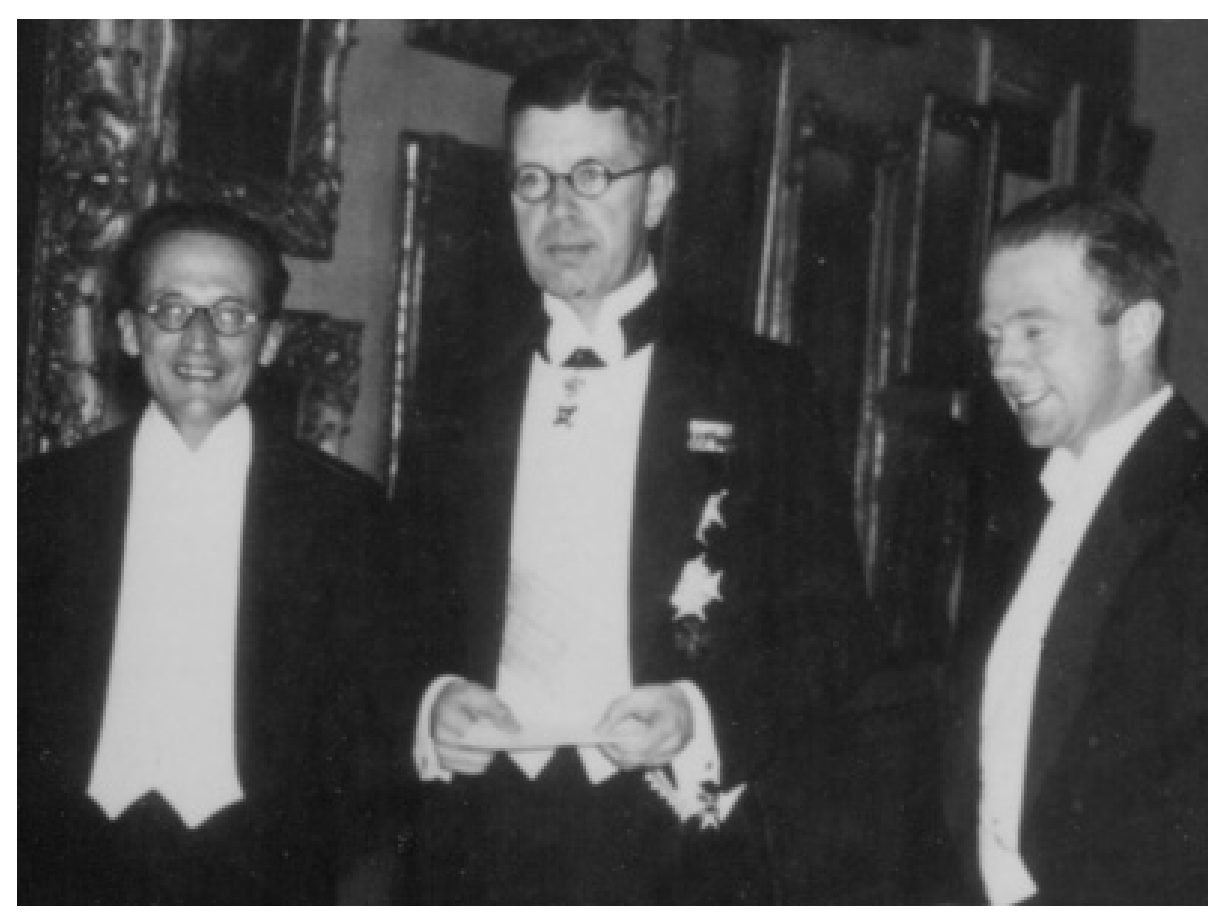
\includegraphics[clip,width=8cm]{Operators/1933hei-sch.ps}
\caption{1933年,薛定谔与海森堡在诺贝尔颁奖典礼上。}
\end{center}
\end{figure}

在已知波函数$\psi$情况下,力学量算符的平均值:$\left\langle {\hat F} \right\rangle  \equiv \overline F  = \int {\psi ^* \hat F\psi dx} $就对应力学量的观测值。

假设在波函数$\psi$下,力学量$F$有唯一确定的值,记作$\overline F $,则力学量的均方偏差(涨落)$\overline {\left( {\Delta F} \right)^2 } $也应为0。

平均值的偏差用算符表示:$\Delta \hat F = \hat F - \overline F $

均方偏差的算符:$\left( {\Delta \hat F} \right)^2  = \left( {\hat F - \overline F } \right)^2 $, 力学量$F$用厄密算符$\hat F$表示,$\hat F^ +   = \hat F$,$ \Rightarrow \Delta \hat F^ +   = \Delta \hat F$

$\overline {\left( {\Delta F} \right)^2 }  = \int {\psi ^* \left( {\Delta \hat F} \right)^2 } \psi dx = \int {\left( {\Delta \hat F\psi } \right)^* \left( {\Delta \hat F\psi } \right)} dx = \int {\left| {\Delta \hat F\psi } \right|} ^2 dx = 0$

$\Delta \hat F\psi  = 0, \Rightarrow \left( {\hat F - \overline F } \right)\psi  = 0$

即:$\hat F\psi  = \overline F \psi $,由于$F$在波函数$\psi$下有唯一确定的值,不妨令:$\overline F  = F$


方程:$\hat F\psi  = F\psi
$,称为本征方程(Eigenequation)\footnote{Eigen在德语中是自己(self)的意思。}。

\index{Eigenequation: 本征方程}

数学上把求解这类方程的问题称为本征值问题(Eigenvalue
problem),方程的解称为本征函数(Eigenfunction),对应的实数称为本征值(Eigenvalue)。
本征值就是力学量可能取的数值,在本征函数代表的本征态中,力学量只能取唯一确定的数值,即本征函数对应的本征值。
通常本征值可以完全分立取值(分立谱,如:线性谐振子),连续取值(连续谱,如:平面波),
分段连续取值(分段连续谱,如:固体能带结构),或分立连续兼而有之(有限深势阱)。

\index{Eigenvalue problem: 本征值问题}

\index{Eigenfunction: 本征函数}

\index{Eigenvalue: 本征值}

可以证明:在任何状态下厄密算符的本征值都是实数;

\index{Hermitian operator: 厄米算符}

$\overline F = \left( {\psi ,\hat F\psi } \right) = \left( {\hat F^
+  \psi ,\psi } \right) = \left( {\hat F\psi ,\psi } \right) =
\left( {\psi ,\hat F\psi } \right)^*  = \overline F ^* $,$
\Rightarrow \overline F  \in {\rm{Real}}$

且其逆定理:在任何状态下平均值为实数的算符必为厄密算符,也成立。

任意$\psi$,$\overline F  = \overline F ^* $,即:$\left( {\psi ,\hat F\psi } \right) = \left( {\psi ,\hat F\psi } \right)^*  = \left( {\hat F\psi ,\psi } \right) = \left( {\hat F^ +  \psi ,\psi } \right)$,$ \Rightarrow \hat F = \hat F^ +  $ ,即$\hat F$是厄密算符;


\subsection{量子力学关于力学量与算符的基本假设}

(1)实验上可观测的力学量,要求其算符的平均值为实数,因此量子力学中表示力学量的算符都是厄密算符;

(2)厄密算符的本征函数组成完全系: 任一函数$\psi \left( x
\right)$可按正交归一本征函数$\left\{ {\phi _n \left( x \right)}
\right\}$展开为级数:$\psi \left( x \right) = \sum\limits_n {c_n
\phi _n \left( x \right)} $,$c_n = \int {\phi _n ^* \left( x \right)\psi \left( x \right)dx}$。证明如下:

\index{Orthonormal basis: 正交归一基}

$\int {\phi _n ^* \left( x \right)\psi \left( x \right)dx} = 
\int {\phi _n ^* \left( x \right)\sum\limits_m {c_m \phi _m \left( x
\right)dx} } = \sum\limits_m {c_m \int {\phi _n ^* \left( x
\right)} \phi _m \left( x \right)dx} 
=  \sum\limits_m {c_m \delta _{n,m} }  = c_n$


(3)当系统处于波函数$\psi$所描写的状态时,
测量力学量$F$所得数值,必为算符$\hat F$的本征值$\left\{ {\lambda _n
} \right\}$之一,测得某个本征值$\lambda _n $的几率为$\left| {c_n }
\right|^2 $。($c_n$常被称为几率振幅)

$\int {\psi ^* \psi dx}  = \int {\left( {\sum\limits_m {c_m \phi _m } } \right)^* \left( {\sum\limits_n {c_n \phi _n } } \right)dx}  = \sum\limits_{m,n} {c_m ^* c_n \int {\phi _m ^* \phi _n dx} }  = \sum\limits_{m,n} {c_m ^* c_n \delta _{m,n} }  = \sum\limits_n {\left| {c_n } \right|^2 }  = 1$

$\overline F  = \int {\psi ^* \hat F\psi dx}  = \int {\left(
{\sum\limits_m {c_m \phi _m } } \right)^* \hat F\left(
{\sum\limits_n {c_n \phi _n } } \right)dx}  = \sum\limits_{m,n} {c_m
^* c_n \lambda _n \int {\phi _m ^* \phi _n dx} }\\
 = \sum\limits_{m,n} {c_m ^* c_n \lambda _n \delta _{m,n} }  = \sum\limits_n {\left| {c_n } \right|^2 \lambda _n } $

如$\hat F$的本征值由分立谱和连续谱共同构成,则$\hat F$的全部本征函数由$\phi _n (x)$和$\phi _\lambda  (x)$构成完全系:$\psi (x) = \sum\limits_n {c_n \phi _n (x)}  + \int {c_\lambda  \phi _\lambda  (x)d\lambda } $,

$\int {\phi _\lambda  ^* (x)\phi _{\lambda '} (x)dx}  = \delta \left( {\lambda  - \lambda '} \right)$



$c_\lambda   = \int {\phi _\lambda  ^* (x)\psi (x)dx}
  = \int {dx\phi _\lambda  ^* (x)\int {c_{\lambda '} \phi _{\lambda '} (x)d\lambda '} }  = \int {d\lambda 'c_{\lambda '} \int {\phi _\lambda  ^* (x)} } \phi _{\lambda '}
  (x)dx\\
  = \int {d\lambda 'c_{\lambda '} \delta \left( {\lambda  - \lambda '} \right)}  = c_\lambda$

归一化:$\sum\limits_n {\left| {c_n } \right|^2 }  + \int {\left| {c_\lambda  } \right|^2 d\lambda }  = 1$


力学量平均值:$\overline F  = \sum\limits_n {\lambda _n \left| {c_n } \right|^2 }  + \int {\lambda \left| {c_\lambda  } \right|^2 d\lambda } $


\subsection{不确定原理的严格证明}

\index{Uncertainty principle: 不确定原理}

设体系是力学量$A$的本征态(波函数$\psi$是算符$\hat A$的本征函数),则测量值为一确定值,即相应本征值,而不会出现涨落,即$\overline {\left( {\Delta A} \right)^2 }  = 0$。若在此波函数下继续测量力学量$B$,由于$\psi$不一定是算符$\hat B$的本征函数,但$\psi$可按照算符$\hat B$正交归一本征函数系展开为级数,所以对应力学量$B$的可能取值应是算符$\hat B$的一系列本征值,这样力学量$B$ 的测量值就不是确定的,而应存在一定的涨落$\overline {\left( {\Delta B} \right)^2 }  \ne 0$。

设两个任意力学量$A,B$,考虑积分:$I\left( \xi  \right) = \int {\left| {\xi \hat A\psi  + i\hat B\psi } \right|^2 dx} $, $\xi  \in {\rm{Real}}$, $\hat A^ +   = \hat A,\hat B^ +   = \hat B$

\begin{center}
$\begin{array}{l}
 I\left( \xi  \right) = \int {\left| {\xi \hat A\psi  + i\hat B\psi } \right|^2 dx}  = \left( {\xi \hat A\psi  + i\hat B\psi ,\xi \hat A\psi  + i\hat B\psi } \right) \\
  = \xi ^2 \left( {\hat A\psi ,\hat A\psi } \right) + i\xi \left( {\hat A\psi ,\hat B\psi } \right) - i\xi \left( {\hat B\psi ,\hat A\psi } \right) + \left( {\hat B\psi ,\hat B\psi } \right) \\
  = \xi ^2 \left( {\psi ,\hat A^2 \psi } \right) + i\xi \left( {\psi ,\left[ {\hat A,\hat B} \right]\psi } \right) + \left( {\psi ,\hat B^2 \psi } \right) \\
 \end{array}$
\end{center}

定义:$\left[ {\hat A,\hat B} \right] = i\hat C$,

$\hat C^ +   = \left[ {\frac{1}{i}\left( {\hat A\hat B - \hat B\hat A} \right)} \right]^ +   =  - \frac{1}{i}\left( {\hat B\hat A - \hat A\hat B} \right) = \hat C$

$I\left( \xi  \right) = \xi ^2 \left( {\psi ,\hat A^2 \psi } \right) - \xi \left( {\psi ,\hat C\psi } \right) + \left( {\psi ,\hat B^2 \psi } \right) = \xi ^2 \overline {A^2 }  - \xi \overline C  + \overline {B^2 }  \ge 0$

$\left( {\overline C } \right)^2  - 4\left( {\overline {A^2 } } \right)\left( {\overline {B^2 } } \right) \le 0$, $\left( {\overline {A^2 } } \right)\left( {\overline {B^2 } } \right) \ge \frac{1}{4}\left( {\overline C } \right)^2 $, $\sqrt {\left( {\overline {A^2 } } \right)\left( {\overline {B^2 } } \right)}  \ge \frac{1}{2}\left| {\overline C } \right| = \frac{1}{2}\left| {\overline {\left[ {\hat A,\hat B} \right]} } \right|$

如定义:$\Delta \hat A = \hat A - \overline A ,\Delta \hat B = \hat B - \overline B $,$\left[ {\Delta \hat A,\Delta \hat B} \right] = \left[ {\hat A,\hat B} \right]$

因此:

\begin{equation}\label{unceratinty principle strict}
\sqrt {\left( {\overline {\Delta A^2 } } \right)\left( {\overline
{\Delta B^2 } } \right)}  \ge \frac{1}{2}\left| {\overline {\left[
{\hat A,\hat B} \right]} } \right|
\end{equation}


简记为:$\Delta A \cdot \Delta B \ge \frac{1}{2}\left| {\overline
{\left[ {A,B} \right]} } \right|$。

例:$A = x,B = p_x ,\left[ {\hat x,\hat p_x } \right] = i\hbar $, $\Delta x\Delta p_x  \ge {\raise0.7ex\hbox{$\hbar $} \!\mathord{\left/
 {\vphantom {\hbar  2}}\right.\kern-\nulldelimiterspace}
\!\lower0.7ex\hbox{$2$}}$


\subsubsection{另一种证法}


对力学量$A$, 期望值$\left\langle A \right\rangle$, 定义新算符:

\begin{equation*}
    \Delta A = A - \left\langle A \right\rangle
\end{equation*}


${\left( {\Delta A} \right)^2
}$的期望值描述了$A$的测量值对$A$的期望值的偏离,

\begin{equation*}
\left\langle {\left( {\Delta A} \right)^2 } \right\rangle  =
\left\langle {A^2 } \right\rangle  - \left\langle A \right\rangle ^2
\end{equation*}

利用施瓦茨不等式(The Schwarz inequality),

\begin{equation*}
\left| {\vec a} \right|^2 \left| {\vec b} \right|^2  \ge \left|
{\vec a \cdot \vec b} \right|^2
\end{equation*}

即:

\begin{equation*}
   \left\langle {\alpha }
 \mathrel{\left | {\vphantom {\alpha  \alpha }}
 \right. \kern-\nulldelimiterspace}
 {\alpha } \right\rangle \left\langle {\beta }
 \mathrel{\left | {\vphantom {\beta  \beta }}
 \right. \kern-\nulldelimiterspace}
 {\beta } \right\rangle  \ge \left| {\left\langle {\alpha }
 \mathrel{\left | {\vphantom {\alpha  \beta }}
 \right. \kern-\nulldelimiterspace}
 {\beta } \right\rangle } \right|^2
\end{equation*}

我们可证明对力学量$A$和力学量$B$, 满足这样的关系:


\begin{equation*}
\left\langle {} \right|\Delta A\Delta A\left| {} \right\rangle
\left\langle {} \right|\Delta B\Delta B\left| {} \right\rangle  \ge
\left| {\left\langle {} \right|\Delta A\Delta B\left| {}
\right\rangle } \right|^2
\end{equation*}


即:

\begin{equation}\label{AB schwarz}
\left\langle {\left( {\Delta A} \right)^2 } \right\rangle
\left\langle {\left( {\Delta B} \right)^2 } \right\rangle  \ge
\left| {\left\langle {\Delta A\Delta B} \right\rangle } \right|^2
\end{equation}


考虑到,

\begin{equation*}
\Delta A\Delta B = \frac{1}{2}[\Delta A,\Delta B] + \frac{1}{2}\{
\Delta A,\Delta B\}
\end{equation*}

这里: $ [\Delta A,\Delta B] = [A,B] $,
并且$[A,B]$是反厄米的(anti-Hermitian), 即:

\index{anti-Hermitian: 反厄米的}

\begin{equation*}
\left( {[A,B]} \right)^\dag   = \left( {AB - BA} \right)^\dag   = BA
- AB =  - [A,B]
\end{equation*}

类似可证$\{ \Delta A, \Delta B\}$是厄米的(Hermitian)。 对厄米算符(即
$A^\dag$ = A)而言, 期望值是纯实数, 因为: $ \left( {\psi ,A\psi }
\right) = \left( {A^\dag  \psi ,\psi } \right) = \left( {A\psi ,\psi
} \right) = \left( {\psi ,A\psi } \right)^* $; 对反厄米算符(即
$A^\dag = -A$)而言, 期望值是纯虚数, 因为: $ \left( {\psi ,A\psi }
\right) = \left( {A^\dag  \psi ,\psi } \right) =  - \left( {A\psi
,\psi } \right) = - \left( {\psi ,A\psi } \right)^* $。

因此$ \Delta A\Delta B$的期望值是一个纯虚数加上一个纯实数:

\begin{equation*}
\left\langle {\Delta A\Delta B} \right\rangle  =
\frac{1}{2}\left\langle {[A,B]} \right\rangle  +
\frac{1}{2}\left\langle {\{ \Delta A,\Delta B\} } \right\rangle
\end{equation*}

所以模方就是虚部平方加实部平方:

\begin{equation*}
\left| {\left\langle {\Delta A\Delta B} \right\rangle } \right|^2  =
\frac{1}{4}\left| {\left\langle {[A,B]} \right\rangle } \right|^2  +
\frac{1}{4}\left| {\left\langle {\{ \Delta A,\Delta B\} }
\right\rangle } \right|^2
\end{equation*}


考虑式\ref{AB schwarz}, 得到:

\begin{equation*}
\left\langle {\left( {\Delta A} \right)^2 } \right\rangle
\left\langle {\left( {\Delta B} \right)^2 } \right\rangle  \ge
\frac{1}{4}\left| {\left\langle {[A,B]} \right\rangle } \right|^2
\end{equation*}


两边分别开根号, 就是不确定原理\ref{unceratinty principle strict}。


\subsection{共同本征函数}


如:$\left[ {A,B} \right] = 0$,$\Delta A \cdot \Delta B = 0$,两力学量可同时取确定的值,可求得$A,B$的共同本征态;

\index{Simultaneous eigenstate: 共同本征态}

设:$\hat A\psi _n  = A_n \psi _n $,$\psi _n$是$\hat A$的本征态,相应本征值为$A_n$

(1)设$A_n$不简并

$\hat A\left( {\hat B\psi _n } \right) = \hat B\hat A\psi _n  = \hat B A_n \psi _n  = A_n \hat B\psi _n $
$ \Rightarrow \hat B\psi _n  = B_n \psi _n $,$\psi _n$本身即构成$\hat A, \hat B$的共同本征态;

(2)设$A_n$,$f_n$重简并

即:$\hat A\psi _{n\alpha }  = A_n \psi _{n\alpha } ,(\alpha  = 1,2,...,f_n )$

$\hat A\left( {\hat B\psi _{n\alpha } } \right) = \hat B\hat A\psi _{n\alpha }  = \hat BA_n \psi _{n\alpha }  = A_n \left( {\hat B\psi _{n\alpha } } \right)$

即$\hat B\psi _{n\alpha } $仍为$\hat A$的本征态,且对应本征值为$A_n$,所以$\hat B\psi _{n\alpha } $是$\psi _{n\alpha '} $的线性迭加;

$\hat B\psi _{n\alpha }  = \sum\limits_{\alpha '} {B_{\alpha '\alpha } \psi _{n\alpha '} } ,(\alpha ' = 1,2,...,f_n )$, $B_{\alpha '\alpha }  = \left( {\psi _{n\alpha '} ,\hat B\psi _{n\alpha } } \right)$

一般来说$\psi _{n\alpha } $不是$\hat B$的本征函数,但$\psi _{n\alpha } $的线性迭加可以是$\hat B$的本征态;


$\phi  = \sum\limits_\alpha  {C_\alpha  \psi _{n\alpha } } $是$\psi _{n\alpha } $的线性迭加,显然:$\hat A\phi  = A_n \phi $,是$\hat A$的本征态;

假设$\phi$也是$\hat B$的本征态:$\hat B\phi  = B\phi $

$\hat B\phi  = \sum\limits_\alpha  {C_\alpha  \hat B\psi _{n\alpha } } $,利用:$\hat B\psi _{n\alpha }  = \sum\limits_{\alpha '} {B_{\alpha '\alpha } \psi _{n\alpha '} } $

$\hat B\phi  = \sum\limits_\alpha  {C_\alpha  \hat B\psi _{n\alpha } }  = \sum\limits_{\alpha \alpha '} {C_\alpha  B_{\alpha '\alpha } \psi _{n\alpha '} }  = B\phi  = \sum\limits_{\alpha '} {BC_{\alpha '} \psi _{n\alpha '} } $


$ \Leftarrow $
$\sum\limits_\alpha  {C_\alpha  B_{\alpha '\alpha } }  = BC_{\alpha '} $
$ \Leftarrow $
$\sum\limits_{\alpha  = 1}^{f_n } {\left( {B_{\alpha '\alpha }  - B\delta _{\alpha \alpha '} } \right)C_\alpha  }  = 0$

上式是本征值$B$的$f_n$次幂代数方程,可解出$f_n$个解,记为:$B_\beta  ,(\beta  = 1,2,...,f_n )$

把每个$B_\beta  $代入$\sum\limits_{\alpha  = 1}^{f_n } {\left( {B_{\alpha '\alpha }  - B\delta _{\alpha \alpha '} } \right)C_\alpha  }  = 0$,可求出一组线性迭加系数:$C_{\beta \alpha } ,(\alpha  = 1,2,...,f_n )$

这样可构造出$f_n$个新的波函数$\phi _{n\beta } $,满足:

\begin{center}
$\begin{array}{l}
 \hat A\phi _{n\beta }  = A_n \phi _{n\beta }  \\
 \hat B\phi _{n\beta }  = B_\beta  \phi _{n\beta }  \\
 \end{array}$
\end{center}


$\phi _{n\beta } $是$\hat A,\hat B$的共同本征态;

如本征值$B$的$f_n$次幂代数方程解出有重根,说明本征值还存在简并,重根的个数,就是这个本征值的简并度。这时需要引入新的与 $\hat A, \hat B$都对易的算符$\hat C$,使$\hat A, \hat B, \hat C$的共同本征态无简并\footnote{参考曾谨言《量子力学 卷I》第199页}。

\subsection{常见力学量的本征函数}

(1)动量算符:

$\frac{\hbar }{i}\frac{\partial }{{\partial x}}\psi _{p_x } (x) = p_x \psi _{p_x } (x)$,$\frac{{\psi '}}{\psi } = \frac{{ip_x }}{\hbar }$,$\left( {\ln \psi } \right)^\prime   = \frac{{ip_x }}{\hbar }$,$\ln \psi  = C + {\textstyle{{ip_x  \cdot x} \over \hbar }}$

所以:$\psi _{p_x } (x) = \exp \left( {C + {\textstyle{{ip_x  \cdot x} \over \hbar }}} \right) = C'\exp \left( {{\textstyle{{ip_x  \cdot x} \over \hbar }}} \right)$,$C'$是归一化常数;

$\int {\psi _{p'_x } ^* \psi _{p_x } dx}  = \delta \left( {p'_x  - p_x } \right)$
$ \Rightarrow C' = \frac{1}{{\sqrt {2\pi \hbar } }}$

动量算符归一化本征函数:

\begin{equation}\label{13-1}
\psi _{p_x } (x) = \frac{1}{{\sqrt {2\pi \hbar } }}\exp \left( {{\textstyle{{ip_x  \cdot x} \over \hbar }}} \right)
\end{equation}

动量谱是连续谱,因此将波函数归一化为$\delta$函数;


(2)角动量算符:将在下节中详细讨论;


\subsection*{阅读与思考}


\begin{itemize}

    \item 不确定关系与薛定谔方程:
海森堡的不确定关系:$\Delta x\Delta p \ge
{\raise0.5ex\hbox{$\scriptstyle \hbar $} \kern-0.1em/\kern-0.15em
\lower0.25ex\hbox{$\scriptstyle 2$}}$可以由算符对易式:$ \left[
{\hat{x},\hat{p}} \right] = i\hbar$
推出。但不确定关系仅给出了测量两不对易力学量不确定程度的下限,对其上限并没有给出限制。Michael
J. W. Hall, Marcel Reginatto在\textbf{Journal of Physics A}发表文章,
认为在严格的不确定关系基础上可以得到薛定谔方程。

阅读下列文献,并写出读书报告。


Michael J. W. Hall, Marcel Reginatto, Schrodinger equation from an
exact uncertainty principle,
\url{http://cn.arxiv.org/abs/quant-ph/0102069}


Adrian Cho, Researchers Race to Put the Quantum Into Mechanics,
\url{http://www.sciencemag.org/cgi/content/full/299/5603/36}


   \end{itemize}
